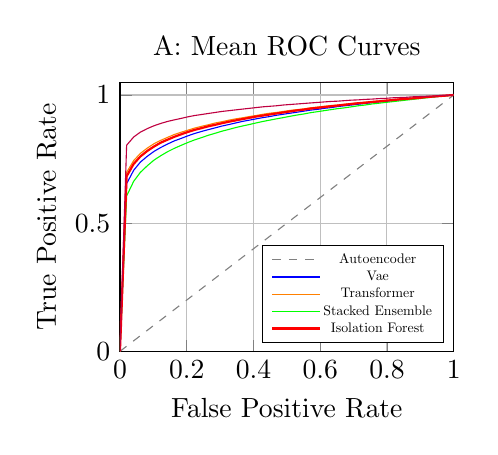
\begin{tikzpicture}
\begin{axis}[
    width=0.48\columnwidth, height=5cm,
    xlabel={False Positive Rate}, ylabel={True Positive Rate},
    xmin=0, xmax=1, ymin=0, ymax=1.05,
    legend pos=south east, legend style={nodes={scale=0.5, transform shape}},
    grid=both, title={A: Mean ROC Curves}]
\addplot [dashed, black!50, domain=0:1] {x};
\addplot [color=blue, mark=none] coordinates {(0.000,0.000) (0.020,0.654) (0.041,0.706) (0.061,0.738) (0.082,0.761) (0.102,0.780) (0.122,0.795) (0.143,0.809) (0.163,0.821) (0.184,0.831) (0.204,0.841) (0.224,0.850) (0.245,0.858) (0.265,0.865) (0.286,0.872) (0.306,0.879) (0.327,0.885) (0.347,0.891) (0.367,0.897) (0.388,0.902) (0.408,0.907) (0.429,0.912) (0.449,0.916) (0.469,0.921) (0.490,0.925) (0.510,0.929) (0.531,0.933) (0.551,0.937) (0.571,0.941) (0.592,0.944) (0.612,0.948) (0.633,0.951) (0.653,0.955) (0.673,0.958) (0.694,0.961) (0.714,0.964) (0.735,0.967) (0.755,0.970) (0.776,0.973) (0.796,0.975) (0.816,0.978) (0.837,0.981) (0.857,0.983) (0.878,0.986) (0.898,0.988) (0.918,0.991) (0.939,0.993) (0.959,0.995) (0.980,0.998) (1.000,1.000)};
\addlegendentry{Autoencoder}
\addplot [color=orange, mark=none] coordinates {(0.000,0.000) (0.020,0.698) (0.041,0.744) (0.061,0.772) (0.082,0.793) (0.102,0.810) (0.122,0.823) (0.143,0.835) (0.163,0.846) (0.184,0.855) (0.204,0.863) (0.224,0.871) (0.245,0.878) (0.265,0.884) (0.286,0.891) (0.306,0.896) (0.327,0.902) (0.347,0.907) (0.367,0.911) (0.388,0.916) (0.408,0.920) (0.429,0.925) (0.449,0.929) (0.469,0.932) (0.490,0.936) (0.510,0.940) (0.531,0.943) (0.551,0.946) (0.571,0.950) (0.592,0.953) (0.612,0.956) (0.633,0.959) (0.653,0.961) (0.673,0.964) (0.694,0.967) (0.714,0.969) (0.735,0.972) (0.755,0.974) (0.776,0.977) (0.796,0.979) (0.816,0.981) (0.837,0.984) (0.857,0.986) (0.878,0.988) (0.898,0.990) (0.918,0.992) (0.939,0.994) (0.959,0.996) (0.980,0.998) (1.000,1.000)};
\addlegendentry{Vae}
\addplot [color=green, mark=none] coordinates {(0.000,0.000) (0.020,0.606) (0.041,0.663) (0.061,0.698) (0.082,0.724) (0.102,0.746) (0.122,0.763) (0.143,0.779) (0.163,0.792) (0.184,0.804) (0.204,0.815) (0.224,0.825) (0.245,0.834) (0.265,0.843) (0.286,0.851) (0.306,0.859) (0.327,0.866) (0.347,0.873) (0.367,0.879) (0.388,0.885) (0.408,0.891) (0.429,0.897) (0.449,0.902) (0.469,0.907) (0.490,0.912) (0.510,0.917) (0.531,0.922) (0.551,0.926) (0.571,0.931) (0.592,0.935) (0.612,0.939) (0.633,0.943) (0.653,0.947) (0.673,0.950) (0.694,0.954) (0.714,0.958) (0.735,0.961) (0.755,0.965) (0.776,0.968) (0.796,0.971) (0.816,0.974) (0.837,0.977) (0.857,0.980) (0.878,0.983) (0.898,0.986) (0.918,0.989) (0.939,0.992) (0.959,0.995) (0.980,0.997) (1.000,1.000)};
\addlegendentry{Transformer}
\addplot [color=red, thick, mark=none] coordinates {(0.000,0.000) (0.020,0.683) (0.041,0.731) (0.061,0.760) (0.082,0.782) (0.102,0.799) (0.122,0.814) (0.143,0.826) (0.163,0.837) (0.184,0.847) (0.204,0.856) (0.224,0.864) (0.245,0.871) (0.265,0.878) (0.286,0.884) (0.306,0.890) (0.327,0.896) (0.347,0.901) (0.367,0.906) (0.388,0.911) (0.408,0.916) (0.429,0.920) (0.449,0.924) (0.469,0.928) (0.490,0.932) (0.510,0.936) (0.531,0.940) (0.551,0.943) (0.571,0.947) (0.592,0.950) (0.612,0.953) (0.633,0.956) (0.653,0.959) (0.673,0.962) (0.694,0.965) (0.714,0.968) (0.735,0.970) (0.755,0.973) (0.776,0.975) (0.796,0.978) (0.816,0.980) (0.837,0.983) (0.857,0.985) (0.878,0.987) (0.898,0.989) (0.918,0.992) (0.939,0.994) (0.959,0.996) (0.980,0.998) (1.000,1.000)};
\addlegendentry{Stacked Ensemble}
\addplot [color=purple, mark=none] coordinates {(0.000,0.000) (0.020,0.804) (0.041,0.836) (0.061,0.855) (0.082,0.869) (0.102,0.880) (0.122,0.889) (0.143,0.897) (0.163,0.903) (0.184,0.909) (0.204,0.915) (0.224,0.920) (0.245,0.924) (0.265,0.928) (0.286,0.932) (0.306,0.936) (0.327,0.939) (0.347,0.942) (0.367,0.945) (0.388,0.948) (0.408,0.951) (0.429,0.954) (0.449,0.956) (0.469,0.958) (0.490,0.961) (0.510,0.963) (0.531,0.965) (0.551,0.967) (0.571,0.969) (0.592,0.971) (0.612,0.973) (0.633,0.975) (0.653,0.976) (0.673,0.978) (0.694,0.980) (0.714,0.981) (0.735,0.983) (0.755,0.984) (0.776,0.986) (0.796,0.987) (0.816,0.989) (0.837,0.990) (0.857,0.991) (0.878,0.993) (0.898,0.994) (0.918,0.995) (0.939,0.996) (0.959,0.998) (0.980,0.999) (1.000,1.000)};
\addlegendentry{Isolation Forest}
\end{axis}
\end{tikzpicture}